\documentclass[12pt]{article}

% URLs and hyperlinks ---------------------------------------
\usepackage{hyperref}
\hypersetup{
    colorlinks=true,
    linkcolor=blue,
    filecolor=magenta,      
    urlcolor=blue,
}
\usepackage{xurl}
%---------------------------------------------------
\usepackage[inline]{enumitem}
\usepackage{graphicx}
\usepackage{multirow}
\usepackage{float}
\renewcommand{\arraystretch}{1.23}

% adjust a verrrrry big table -------------------------------
\usepackage{adjustbox}
% -----------------------------------------------------------

\usepackage{array}
% center the p columns and m --------------------------------------------------------------
\newcolumntype{P}[1]{>{\centering\arraybackslash}p{#1}}
\newcolumntype{M}[1]{>{\centering\arraybackslash}m{#1}}
% -------------------------------------------------------------------------------------------------------------

\usepackage{xepersian}
\settextfont{Yas}
\setdigitfont{Yas}

\begin{document}
    \begin{titlepage}
        \centering
        \vspace{1cm}
        {\Huge \lr{\textbf{Business Case}}\par}
        \vspace{15mm}
         
\includegraphics{../images/alogo} \par
        
        \vfill \par	\vfill
        
        {\small
        اعضای تیم: \par    
            \itshape                مهدی حق‌وردی\\
            سید محمدحسین هاشمی \par}
        \vspace{5cm}
        {\large مهر ۱۴۰۲\par}
    \end{titlepage}
\tableofcontents
\newpage

\section{خلاصه اجرایی}

\section{مقدمه}
در همه شرکت‌ها برای مشاهده عملکرد کارکنان سازوکارها یا آماری دقیقی وجود دارد که به مدیران گزارشات دقیقی از عملکرد جزئی و کلی کارمندان آن شرکت می‌دهند،‌ و مدیران با استفاده از تحلیل و بررسی این آمار‌ها حقوق، پاداش و حتی برخی نیازهای کارمندان را مورد بررسی قرار می‌دهند و عملکرد کلی شرکت را بهبود می‌بخشند. 

در شرکت‌های کوچک و استارت‌آپ‌ها به دلیل وسعت کاری کم و تعداد پایین کارکنان، این ارزیابی‌ها به طور مستقیم توسط مدیران انجام می‌شود، ولی در شرکت‌هایی مانند \lr{Amazon} به دلیل وسعت جهانی شرکت و همچنین تعداد بسیار زیاد کارمندان چنین امکانی وجود ندارد؛ علاوه بر این، در موقعیت کنونی شرکت \lr{Amazon} هیچ راه‌حل خوبی برای حل این مشکل ارائه نشده و ارائه‌ی یک راه‌حل خوب یکی از نیاز‌های اساسی این شرکت است؛ که در این سند به بررسی راه‌حل‌ها \lr{(Solutions)} و جایگزین‌هایی برای حل این مشکل می‌پردازیم.
\subsection{ساختار شرکت}\label{amz-struct}
در سیستم \lr{Amazon Analytics} شرکت \lr{Amazon} در تصویر \ref{amz-s3} به سه بخش اصلی (و درختی) تقسیم می‌شود.
\begin{figure}[b]
\begin{center}
    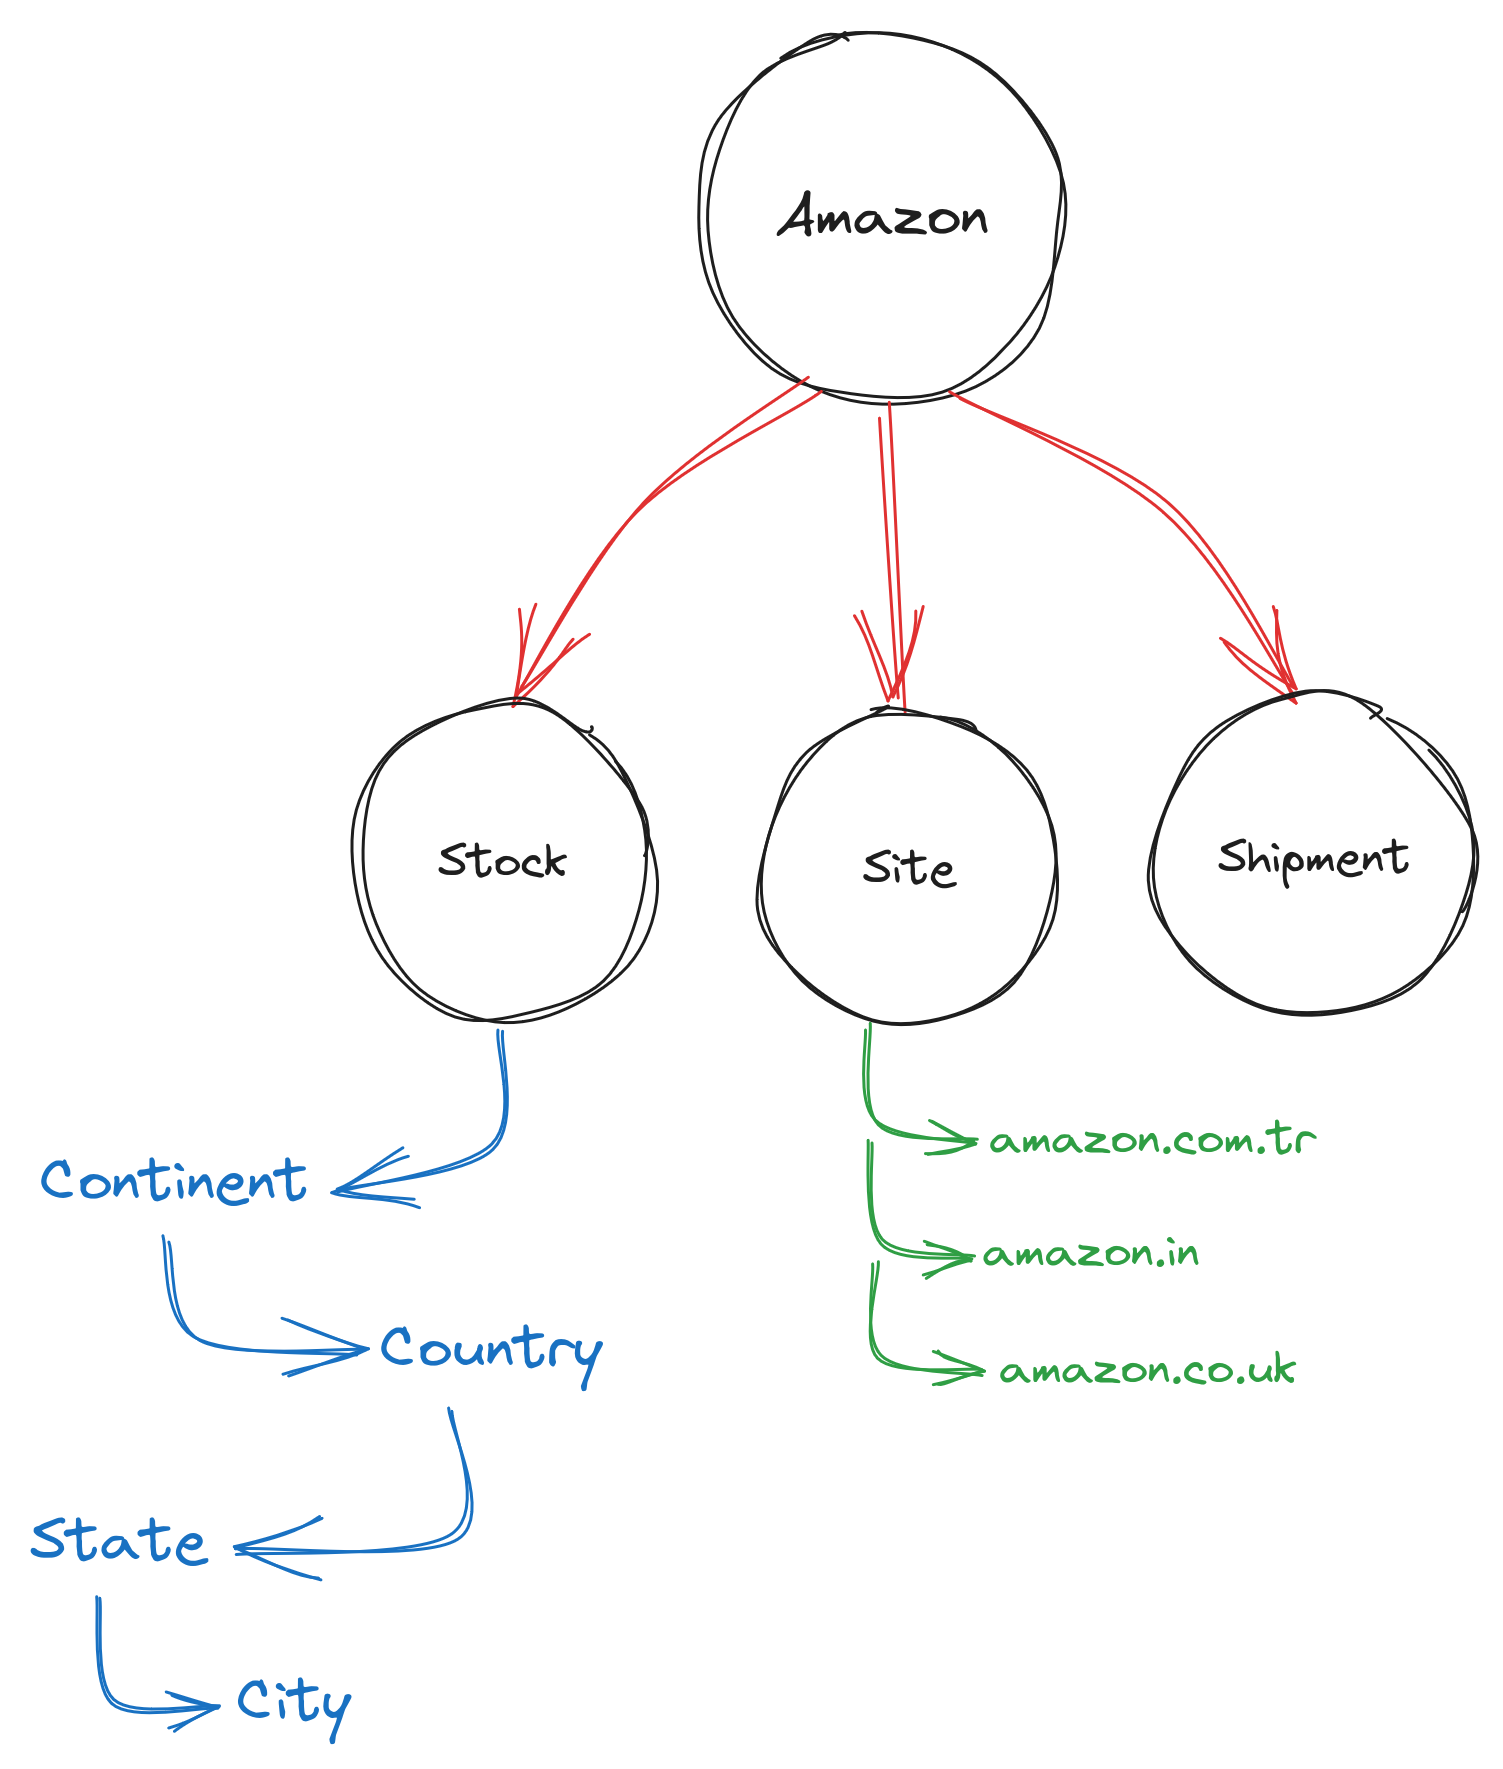
\includegraphics[width=\textwidth, height=\textheight]{../images/amazon-s3-comp(2)}
\end{center} 
\caption{ساختار کلی شرکت \lr{Amazon}}\label{amz-s3}
\end{figure}

\subsection{ارزش‌های قابل‌ اندازه‌گیری}\label{intro-movs}
با توجه به این تقسیم‌بندی انجام شده در \ref{amz-struct}، ارزش‌های قابل‌ اندازه‌گیری \label{movs}
و مهم برای شرکت \lr{Amazon} به شرح زیر می‌باشد:

\begin{itemize}
    \item  انبارداری \lr{(Stock)}
    
    \textbf{هدف اصلی} محصول باید در انبار‌هایی نزدیک محل تحویل باشد.
    \begin{itemize}
        \item 
        کالا‌ها باید در نزدیک‌ترین محل به مقصد ارسال کالا باشند (با \lr{km}\LTRfootnote{\lr{Kilometre}}سنجش می‌شود).
        
        \item 
        زمان پردازش و تحویل کالا به بخش ارسال کالا \lr{(Shipment)}، کمترین زمان ممکن باشد (با دقیقه و ساعت بررسی می‌شود).        
    \end{itemize}
    
    \item وبسایت \lr{Amazon} \lr{(Site)}
    
    \textbf{هدف اصلی} راحتی خرید
    \begin{itemize}
        \item سرعت بارگزاری وبسایت‌های \lr{Amazon} همه‌جا (با ثانیه بررسی می‌شود).
        
        \item 
        طراحی و تجربه‌ی کاربری \lr{(UI/UX)} (بازخورد‌های کیفی کاربران، برای مثال \textit{آیا این صفحه مفید بود} یا \textit{به صفحه‌ی \lr{x} چه امتیازی می‌دهید} و...)
    \end{itemize}

    \item ارسال کالا \lr{(Shipment)}
    
    \textbf{هدف اصلی} محصول سریع و سالم برسد
    \begin{itemize}
        \item 
        زمان تحویل کالا (با تعداد ساعت و روز بررسی می‌شود).
        \item 
        مسافت طی شده‌ی کالا (با \lr{km} سنجش می‌شود).
        
        \item 
        رضایت مشتری برای کالای تحویل داده شده (بازخورد‌های کیفی کاربران، برای مثال 
        \textit{به مامور تحویل چه امتیازی می‌دهید}،
        \textit{آیا کالا سالم است} و سوالاتی از این قبیل).
    \end{itemize}
\end{itemize}

\subsection{\lr{MOV}}
این پروژه موفقیت‌آمیز خواهد بود اگر
\begin{itemize}
    \item 
    بتواند تحلیل و ارزیابیِ تمامی ارزش‌های قابل‌ اندازه‌گیری بالا را به مدیران رده‌بندی‌ شده بر اساس درخت سازمانی گزارش دهد.
    \item 
    بتواند با مقایسه‌ی عملکرد فعلی بخش‌های مختلف شرکت، میزان رشد و بهبود عملکرد آن را به صورت درصدی و دقیق گزارش دهد.
    \item
    مدیران شرکت علاوه‌ بر دسترسی به عملکرد بخش‌های مختلف شرکت، امکان دسترسی به بخش‌های کوچک و حتی هر کارمند را در صورت نیاز داشته باشد.

    \item 
    ارزیابی‌های انجام شده متناسب‌ با خروجی و عملکرد واقعی و قابل مشاهده‌ی شرکت باشد.
\end{itemize}

\textbf{لازم به ذکر است}
 که وظیفه و هدف پروژه صرفا ارزیابی آمار و تحلیل رشد و پیشبینی عملکرد شرکت خواهد بود، پس با این رویه مدیران و کارمندان شرکت \lr{Amazon}خودشان باید به فکر بهبود و ارتقای ارزش‌های قابل اندازه‌گیری ذکر شده باشند.

\section{جایگزین‌ها}
در این بخش، به بررسی جایگزین‌ها و راه‌حل‌های ممکن برای پیاده‌سازی \lr{Amazon Analytics} می‌پردازیم.

\subsection{گزارشات کتبی \lr{(Written Reports)}}\label{written-report}
در این راه‌حل هر کارمند در انتهای شیفت کاری، روز، ماه یا سال گزارشی از عملکرد خود یا بخشی که در آن کار می‌کند، به صورت کتبی به مدیر بخش ارائه می‌دهد. سپس مدیر بخش گزارشات دریافتی از کارمندان زیر دست خود را، جمع‌آوری، ارزیابی و تحلیل می‌کند و پس از آن عملکرد کلی بخش خود و زیردستان خود را به مدیران بالا دستی خود ارائه می‌دهد.
همین روند تا مدیران ارشد شرکت و سهام‌داران ادامه پیدا می‌کند.
\subsection{ارائه کتبی-دیجیتالی \lr{(Half Digital)}}\label{half-digital}
در این روش، ثبت گزارشات \underline{با دست ولی به صورت الکترونیکی} صورت می‌پذیرد.
کارمندان گزارش عملکرد خود و بخش خود را به صورت دیجیتال به مدیران خود ارائه می‌دهند و به تبع آن، مدیران پس از تحلیل گزارشات دریافتی، نتایج آنها را هم به صورت دیجیتالی به مدیران ارشد و بالادستی خود ارائه می‌دهند.
\subsection{ارزیابی دیجیتالی \lr{(Full Digital)}}\label{full-digital}
در این روش، تمامی داده‌ها و آمار‌های کارمندان، بخش‌ها و مدیران شرکت، به علاوه‌ی بازخورد‌های کاربران به صورت کاملا دیجیتالی و بدون دخالت دست انسان، جمع‌آوری شده و سپس تمامی تحلیل‌ها و ارزیابی‌های آنها در سیستم \lr{Amazon Analytics} انجام شده و به صورت کاملا طبقه بندی شده به تمامی مدیران ارائه می‌گردد.

\subsection{بررسی یک مثال با راه‌حل‌های مختلف}
برای مثال می‌خواهیم تحویل یک کالا را از جهات مختلف بررسی کنیم.
\begin{itemize}
    \item راهکار \ref{written-report}
    
    مامور تحویل 
    \begin{enumerate*}
        \item 
        ساعت دریافت،
        \item 
        مسافت طی شده و 
        \item 
        ساعت تحویل کالا
    \end{enumerate*}
     را \textbf{شخصا} و به صورت \textbf{کتبی} پس از هر تحویل، در برگه‌ی گزارش روزانه‌ی خود مکتوب کرده و در پایان شیفت کاری، به مدیر بخش خود تحویل می‌دهد.
    
    سپس مدیر بخش، ارزیابی‌های مامورین مختلف را جمع‌آوری و تحلیل کرده و تمامی تحلیل‌های خود را به صورت \textbf{کتبی} به مدیران بالادستی خود ارائه می‌دهد.
    
    \item راهکار \ref{half-digital}
    
       مامور تحویل 
       \begin{enumerate*}
           \item 
           ساعت دریافت،
           \item 
           مسافت طی شده و 
           \item 
           ساعت تحویل کالا
       \end{enumerate*}
       را \textbf{شخصا} و به صورت \textbf{دیجیتالی} پس از هر تحویل، در برگه‌ی گزارش دیجیتالی روزانه‌ی خود ثبت کرده و در پایان شیفت کاری، برای مدیر بخش خود ارسال می‌کند.
       
    مدیر بخش در این روش، تحلیل‌ و آمار‌های دریافتی از کارمندان خودش را به صورت دیجیتال به مدیران بالادستی خود ارائه می‌دهد.
    
    در این روش برخلاف روش \ref{written-report} مدیران بالادستی درگیر تحلیل و آمار کاغذی نشده و از مزایای دیجیتالی بودن گزارشات (مثل دسته بندی راحت‌تر، قابلیت جستجو‌ی راحت‌تر و...) بهره‌مند می‌شوند.
    \item راهکار \ref{full-digital}
    
    زمانی که مامور تحویل، کالایی را برای تحویل به مشتری دریافت می‌کند، به صورت خودکار زمان دریافت کالا به مامور، مسافت طی شده و زمان تحویل کالا به مشتری، در سیستم ثبت شده و این آمار به صورت لحظه‌‌ای برای مدیران بالادستی قابل دسترسی می‌باشد.
    
    در این روش، دریافت اطلاعات، ارزیابی و تحلیل آنها به عهده‌ی سیستم است و هیچ کاربری در آن امکان دخالت ندارد. 
    
    در روش برخلاف \ref{half-digital} که وظیفه‌ی تحلیل آمار دریافتی به عهده‌ی مدیر بخش بود، تمامی تحلیل‌ها به صورت سیستمی انجام می‌شود و مدیران به راحتی به \textbf{خروجی} و \textbf{نتایج} تحلیل‌ها دسترسی آنی دارند.
    
\end{itemize}

\section{تحلیل جایگزین‌ها}
در این قسمت به بررسی راه‌حل‌های ارائه می‌پردازیم و جنبه‌های متفاوت‌ آنها را بررسی می‌کنیم.

\begin{itemize}
\item         
روش‌های جمع‌آوری داده
\begin{itemize}
    \item راهکار \ref{written-report} 
    
    کاملا دستی، و به صورت پایین به بالا انجام می‌شود.
  
  در این روش، تا زمانی که کارمندی گزارشات خود را مکتوب نکرده و تحویل نداده، هیچ مدیری به هیچ داده‌ی جدیدی دسترسی نداشته؛ به علاوه گزارشات دریافتی از کارمندان و تحلیل‌ها میتوانند کاملا غیرواقعی‌ باشند.
    \item راهکار \ref{half-digital}
    
    ارائه گزارشات اولیه و عملکرد پایه‌ای هر کارمند به صورت دستی ولی دیجیتال و پایین به بالا انجام می‌شود.
    
    در این روش برخلاف روش \ref{written-report} گزارشات دیجیتال دریافت می‌شوند اما همانند روش \ref{written-report} تا زمانی که کارمندی گزارشات خود را ثبت نکرده، هیچ مدیری به هیچ داده‌ی جدیدی دسترسی ندارد. به علاوه، در این روش چون ثبت اطلاعات به صورت دیجیتال صورت می‌گیرد، دسترسی به گزارشات گذشته راحت‌تر و دقیق‌تر از روش \ref{written-report} است.
    
    \item راهکار \ref{full-digital}
    
    تمامی آمار و اطلاعات به صورت خودکار توسط سیستم محاسبه و ثبت می‌شود و کاربر هیچ دخالتی در آن ندارد.
    
    در این روش، امکان جعل آمار و تغییر آن به هیچ عنوان وجود ندارد و مدیران (در صورت نیاز) به صورت تماما لحظه‌ای، می‌توانند ارزیابی و گزارشات آماری و عملکرد کارمندان و بخش‌های مختلف شرکت را از سیستم دریافت کنند.
\end{itemize}
\item         
متریک‌های مورد استفاده

تمامی این متریک‌ها در \ref{intro-movs} و در تصویر \ref{amz-comp} تعریف شده‌اند.

\begin{figure}[b]
    \begin{center}
        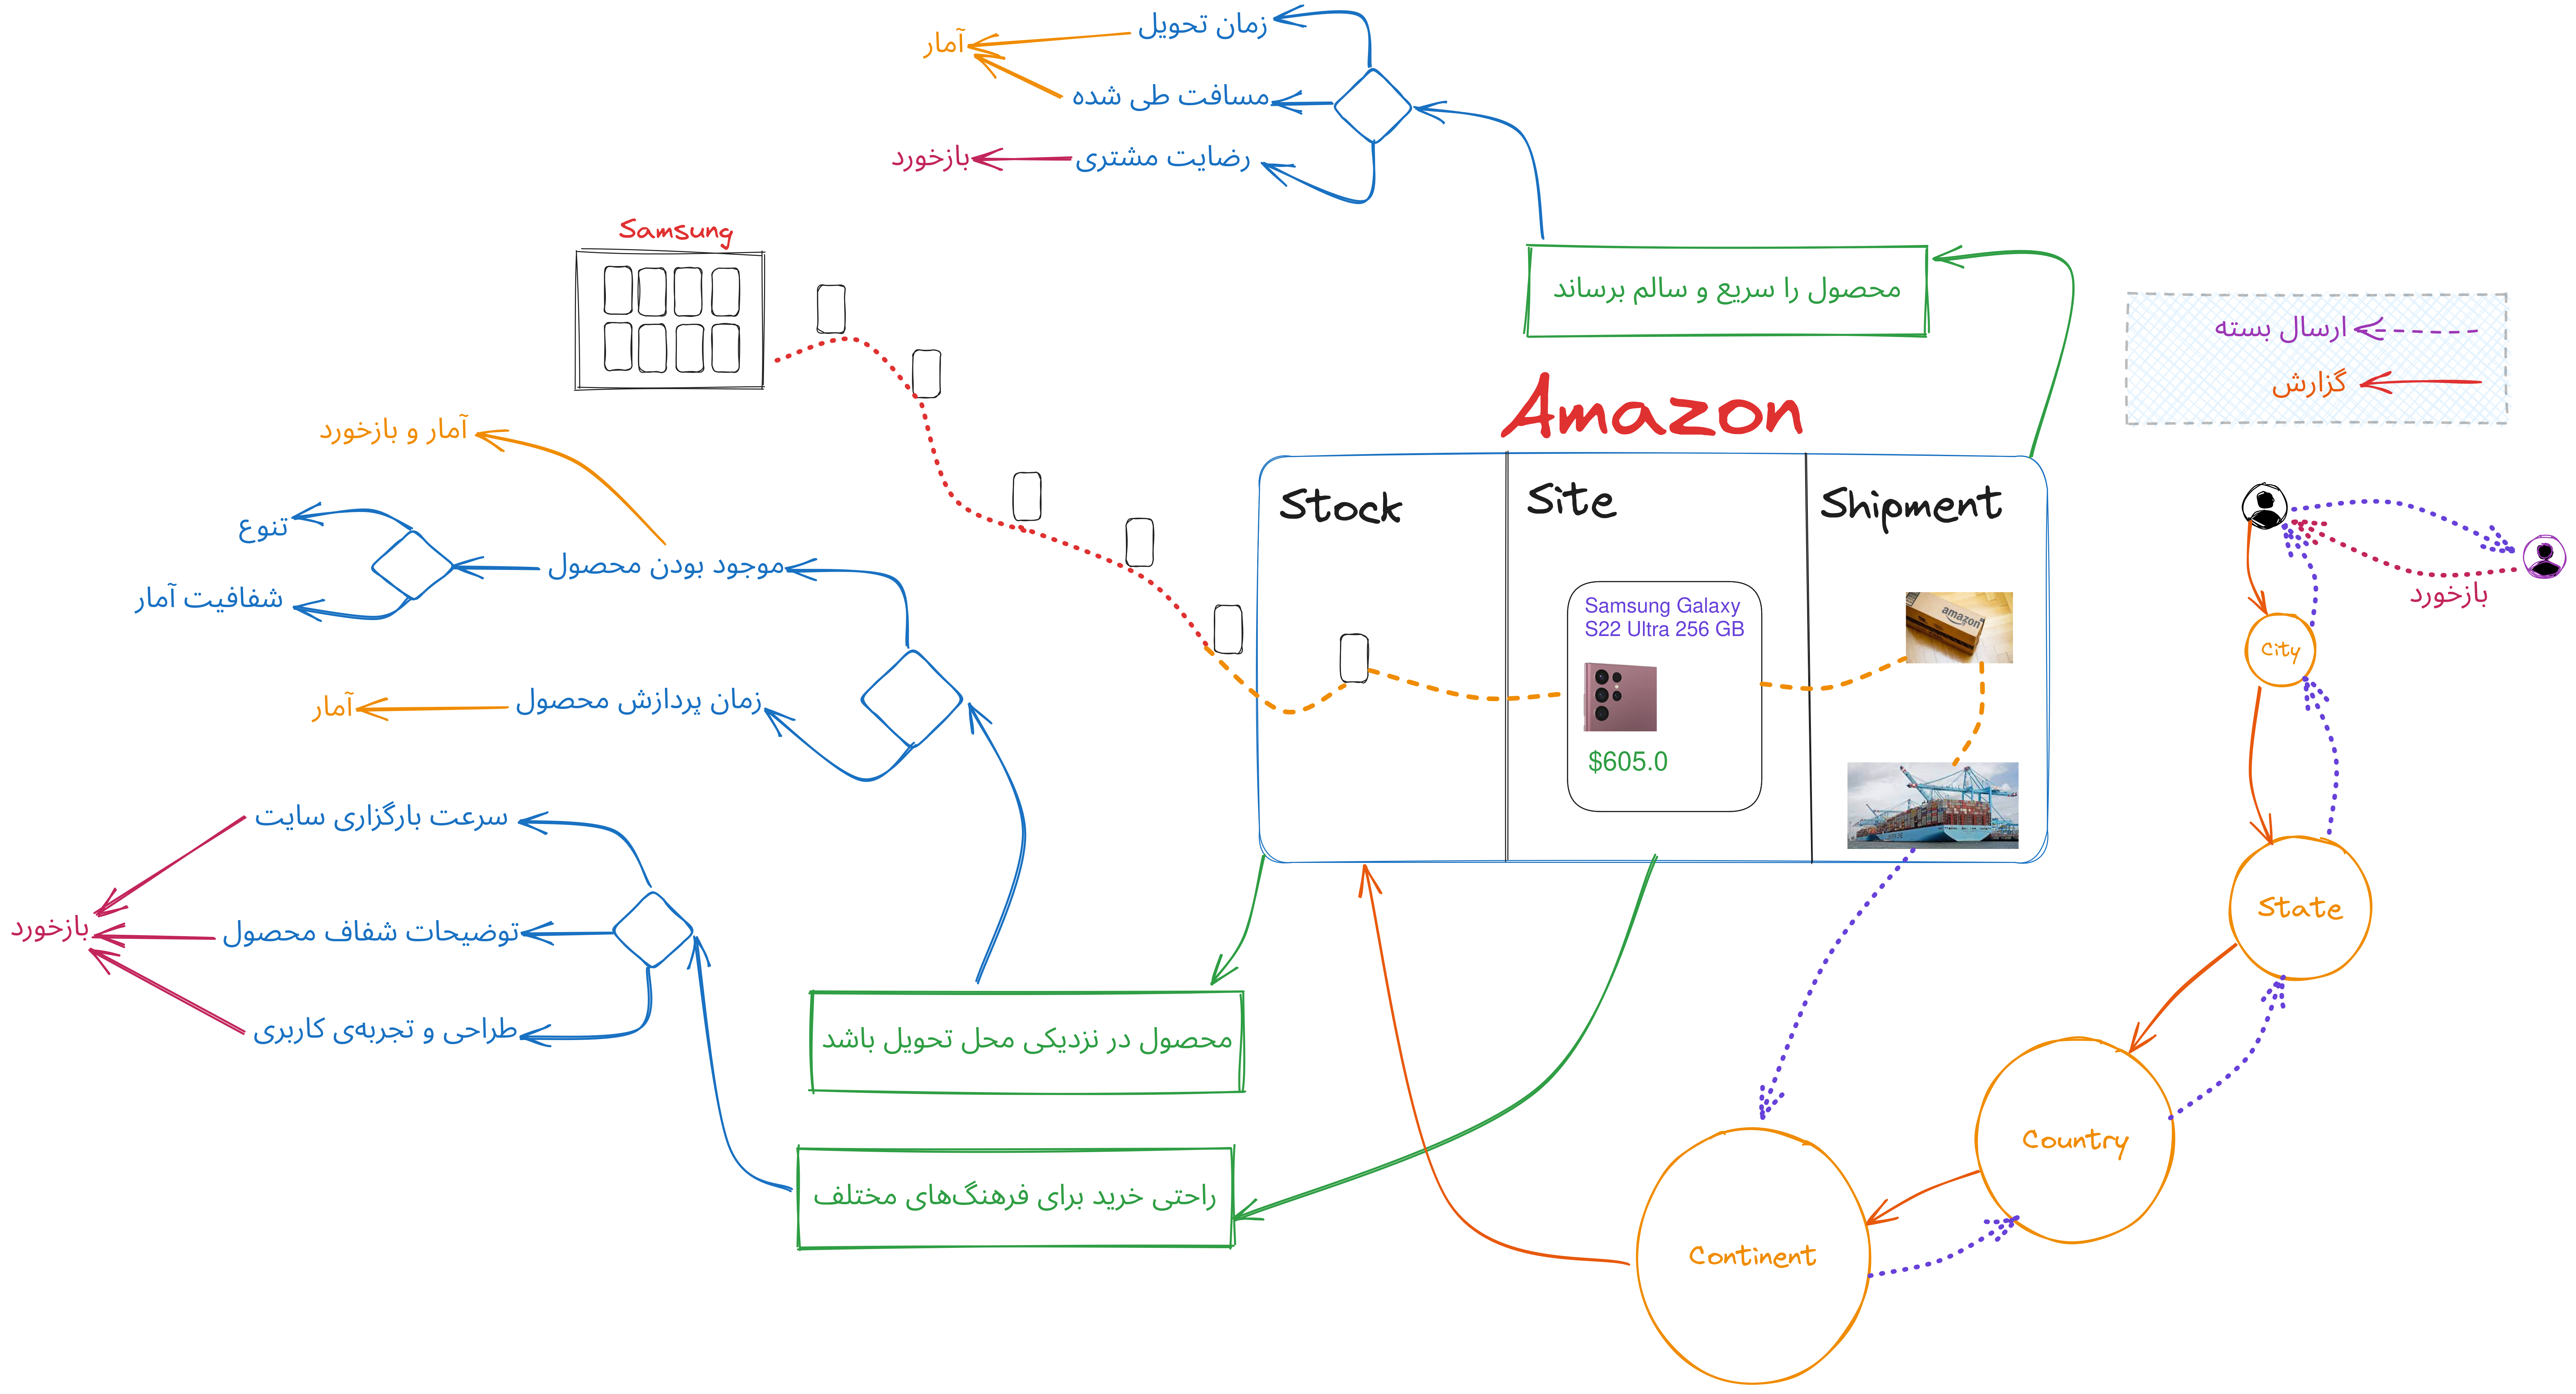
\includegraphics[width=\textheight, height=\textwidth, angle=90]{../images/amazon-comp(2)}
    \end{center}
\caption{ارزش‌ها و متریک‌های مهمِ \lr{Amazon Analytics}}\label{amz-comp}
\end{figure}
\end{itemize}

\subsection{ارائه نتایج بررسی و مقایسه}
\begin{table}[H]\caption{\lr{Does the strategy meet the required objectives?}}
    \begin{latin}
        \begin{center}
            \begin{adjustbox}{width=\textwidth}
                \begin{tabular}{|M{4cm}|c|M{4cm}|c|}
                    \hline
                    \multirow{2}{*}{Required Objectives}
                    & \multicolumn{3}{|c|}{Strategies} \\
                    \cline{2-4}
                    & Written Reports (\ref{written-report}) & Half Digital (\ref{half-digital}) & Full Digital (\ref{full-digital}) \\
                    \hline
                    \rl{دسترسی به عملکرد همه بخش‌ها توسط مدیران} & Yes, but hard & Yes  & Yes \\
                    \hline
                    \rl{دریافت گزارش عملکرد در بازه‌های کوتاه مدت و یا آنی} &  No & Yes, but if user submits them quickly & Yes \\
                    \hline
                    \rl{اعتبار ارزیابی} & No & No & Yes \\
                    \hline
                \end{tabular}
            \end{adjustbox}
        \end{center}
    \end{latin}
\end{table}
\end{document}